\documentclass{article}
\usepackage[a4paper,left=2.5cm,right=2.5cm,top=2.5cm,bottom=2.5cm]{geometry}

\title{Session 2 \\
\Large{Auctions and Electronic Markets}
}
\author{Zohaad Fazal}
\date{February 2020}

\usepackage{natbib}
\usepackage{graphicx}
\usepackage{outlines}
\usepackage{tikz}
\usetikzlibrary{arrows.meta}
\usetikzlibrary{decorations.pathmorphing, patterns,shapes}
\usepackage{amsmath}
\usepackage{amssymb}

% derivative symbol
\renewcommand{\d}[1]{\ensuremath{\operatorname{d}\!{#1}}}



\begin{document}
% zigzag
\pgfdeclarepatternformonly{zigzag}
{\pgfpointorigin}{\pgfpoint{1cm}{1cm}}
{\pgfpoint{0.3cm}{0.3cm}}
\maketitle

\section*{Economics}
Sale of 1 indivisible item, $N=\{1,\dots,n\}$ agents, buyers, bidders, players.

\noindent
Each agent $i\in N$ has a valuation $v_i\in [0,1]$ for ownership of the item.

\section*{Topics}
\begin{outline}
    \1 auction formats
        \2 1\textsuperscript{st} price sealed bid
        \2 2\textsuperscript{nd} price sealed bid
    \1 equilibrium concepts
        \2 DSE (Dominant Strategy Equilibrium)
        \2 ex-post/no-regret equilibrium
        \2 BNE (Bayesian Nash Equilibrium)
        
\end{outline}

\section*{Efficiency/Pareto optimality}
\textbf{Aim:} try to allocate to an agent $i\in N$ such that $v_i \geq v_j$ for all $j\in N$. \\

\noindent
\textbf{Problem:} information asymmetry \\
\noindent
Private values: agent $i$ knows $v_i$, but not the valuations of the others. Auctioneer does not know any $v_i$'s.\\

\noindent
\textbf{Task:} can we design 
\begin{itemize}
    \item a market
    \item a negotiation protocol
    \item a trading platform
    \item an auction
\end{itemize}
in such a way that \textit{in equilibrium} the resulting allocation is efficient?\\

\noindent
\textbf{Answer:} yes.

\section*{Auction}
An auction consists of:
\begin{enumerate}
    \item Legal moves (bids)
    \item Allocation
    \item Payments
\end{enumerate}

\section*{Auction Design: Vickrey auction/2\textsuperscript{nd} price, sealed bid auction}


\begin{enumerate}
    \item Bids: each agent submits a single bid $b_i\in[0,1]$ or $b_i(v_i)$ ex-ante (before $v_i$ is known).
    \item Allocate item to an agent $i\in N$ with $b_i\geq b_j$ for any $j\in N$, this is the winner.
    \item Winner $i$ pays $p_i=\max_j \{b_j|j\neq i\}$, for the others, $j\neq i$,  $p_j=0$.
\end{enumerate}

\section*{Theorem (Vickrey)}
Bidding truthfully, $b_i(v_i)=v_i$, is a \textit{dominant strategy} in the Vickrey auction. (dominant strategy: no matter what the other people do, a dominant strategy is a best response to that). In the resulting DSE, the allocation is efficient.\\

\noindent
2 remarks:
\begin{itemize}
    \item Quasi-linear utility: $u_i=v_i-p_i$.
    \item $b_i(v_i)=v_i$ is a dominant strategy; maximizes utility regardless of other bidders' bids.
\end{itemize}

\subsection*{Sketch of proof}


\begin{center}
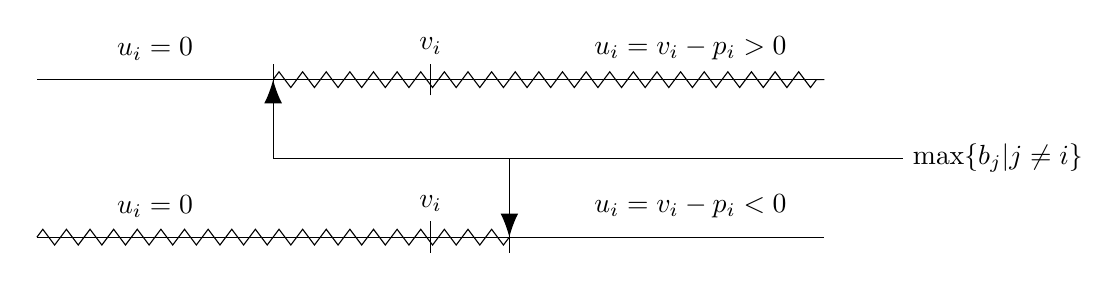
\begin{tikzpicture}


% upper line 
\draw (10,2) -- (0,2) node[label={[xshift=1.5cm]$u_i=0$}] {} node[label={[xshift=8.3cm]$u_i=v_i-p_i>0$}] {};
% left vertical bar
\draw (3, 1.8) -- (3, 2.2);
% middle vertical bar
\draw (5, 1.8) -- (5, 2.2) node[anchor=south] {$v_i$};
% zigzag line
\draw[decoration = {zigzag,segment length = 3mm, amplitude = 1mm},decorate] (3,2)--(10,2);

% middle line
\draw (3,1) -- (11,1) node[right] {$\max\{b_j|j\neq i\}$} ;
% arrow upwards
\draw[[-{Latex[length=3mm]}](3,1) -- (3,2);
% arrow downwards
\draw[[-{Latex[length=3mm]}](6,1) -- (6,0);


% lower line
\draw (0,0) -- (10,0) node[label={[xshift=-1.7cm]$u_i=v_i-p_i<0$}] {} node[label={[xshift=-8.5cm]$u_i=0$}] {};
% right vertical bar
\draw (6, -0.2) -- (6, 0.2);
% middle vertical bar
\draw (5, -0.2) -- (5, 0.2) node[anchor=south] {$v_i$};
% zigzag line
\draw[decoration = {zigzag,segment length = 3mm, amplitude = 1mm},decorate] (0,0)--(6,0);

\end{tikzpicture}
\end{center}

\noindent
{
\tikz\draw[decoration = {zigzag,segment length = 3mm, amplitude = 1mm}, decorate] (0,0) -- ++(0.60,0);
} signifies the best response for bidder $i$. $b_i(v_i)=v_i$ is \textit{always} a best response, and is therefore a dominant strategy.

\section*{Wolf and Sheep}
\subsection*{Ex-post/no-regret equilibrium}
$b_i(v_i)$ defines a \textit{bid strategy}; $v_i\mapsto b_i(v_i)$.\\
\noindent
$b=(b_1,\dots,b_n)$ defines a \textit{bid profile}.\\

\noindent
Profile $b$ is an ex-post equilibrium if for every realization $(v_1,\dots,v_n)$ of valuations the bid profile $(b_1(v_1),\dots,b_n(v_n))$ is a Nash Equilibrium in the auction game.\\

\noindent
\textbf{Wolf:} Bidder 1 is the wolf, $b_1(v_1)=1$. The bid function looks like this:
\begin{center}
\begin{tikzpicture}
\draw[thick,->] (0,0) -- (3,0) node[anchor=north west] {$b_1$} node[anchor=north east] {1};
\draw[thick,->] (0,0) -- (0,3) node[anchor=south east] {$v_1$} node[anchor=north east] {1};
\draw[thick] (0,3) -- (3,3) {};
\end{tikzpicture}
\end{center}

\noindent
\textbf{Sheep:} Bidder $j\neq i$, $b_j(v_j)=0$.\\

\noindent
\textbf{Claim:} Profile $(b_1,\dots,b_n)$ is an ex-post equilibrium.\\

\noindent
\textbf{Proof:} Take any realization $(v_1,\dots,v_n)$. Is the resulting bid profile $(b_1(v_1),\dots,b_n(v_n))=(1,0,\dots,0)$ a Nash Equilibrium?\\

\noindent
\textbf{Wolf:} Bidding against $(0,\dots,0)$, possible utility levels: $u_1=0$ or $u_i=v_1-p_1=v_1$

\noindent
\textbf{Sheep:} Bidding against $(1,0.\dots,0)$, possible utility levels for $j\neq 1$: $u_j=0$ or $u_j=v_j-1\leq0$.

\section*{Auction Design: 1\textsuperscript{st} price, sealed bid auction}

\begin{enumerate}
    \item Bids: each agent submits a bid $b_i\in[0,1]$, $b_i(v_i)$ ex-post.
    \item Allocate item to an agent $i\in N$ (winner) with $b_i\geq b_j$ for any $j\in N$.
    \item Winner $i$ pays $p_i=b_i$.
\end{enumerate}

\section*{Bayesian Nash Equilibrium}

\section*{Intermezzo}
\textbf{Assumptions:} valuations are i.i.d. draws from a uniform distribution on the unit interval [0,1]. 
\noindent
The \textit{copula} (contains the dependence structure between random variables):
\begin{equation*}
v_1
\begin{array}{c}
    \text{L} \\
    \text{H}
\end{array}
\\
\overset
{
    \begin{array}{cc}
    \multicolumn{2}{c}{v_2}\\
    \text{L}   &  \text{H}\\
    \end{array}
}
{
    \left[
        \begin{array}{cc}
        \frac{3}{12} & \frac{1}{12} \\
        \frac{6}{12} & \frac{2}{12} \\
        \end{array}
    \right]
}
\end{equation*}

\begin{equation*}
    \mathbb{P}[v_1=\text{H}, v_2=\text{L}]=\frac{6}{12}
\end{equation*}

\noindent
Are $v_1$ and $v_2$ independent? Multiply the marginals to find out:

\begin{equation*}
    \begin{aligned}
        \mathbb{P}[v_1=\text{H}]\cdot\mathbb{P}[v_2=\text{L}]&=\left(\frac{6}{12}+\frac{2}{12}\right)\cdot\left(\frac{3}{12}+\frac{6}{12}\right)\\
        &=\frac{8}{12}\cdot\frac{9}{12}\\
        &=\frac{2}{3}\cdot\frac{3}{4}=\frac{6}{12}
    \end{aligned}
\end{equation*}
\noindent
So yes, they are independent.

\subsection*{Bayes' Rule}
\begin{equation*}
    \mathbb{P}[v_1=\text{H}|v_2=\text{L}]=\frac{\mathbb{P}[v_2=\text{L}|v_1=\text{H}]\cdot\mathbb{P}[v_1=\text{H}]}{\mathbb{P}[v_2=\text{L}]}
\end{equation*}

\section*{Interim analysis}
\textbf{Claim:} Profile $b=(b_1,\dots,b_n)$ with $b_i(v_i)=\frac{n-1}{n}\cdot v_i$ is a BNE.\\
\noindent
\textbf{Proof:} Take bidder $i$, you know $v_i$ (interim analysis), other bidders $j$ bid $b_j(v_j)=\frac{n-1}{n}\cdot v_j$. Suppose you bid some bid $b$.

\begin{equation*}
\begin{aligned}
    \mathbb{E}(u_i)=(v_i-b)\cdot\mathbb{P}[i \text{ wins}]&=(v_i-b)\cdot \mathbb{P}\left[b>\frac{n-1}{n}v_j\text{ for all }j\neq i\right]\\
    &=(v_i-b)\cdot\mathbb{P}\left[v_j<\frac{n}{n-1}b\text{ for all } j\neq i\right]\\
    &=(v_i-b)\cdot\left(\frac{n}{n-1}b\right)^{n-1}
\end{aligned}
\end{equation*}

\noindent
To maximize, take derivative with respect to $b$, the first order condition is:
\begin{equation*}
    \begin{aligned}
        \frac{\operatorname{d}}{\d b}\mathbb{E}(u_i)&=-1 \cdot \left( \frac{n}{n-1}b \right)^{n-1}+(n-1) \left( \frac{n}{n-1}b \right)^{n-2} \cdot \frac{n}{n-1} \cdot (v_i-b)=0\\
        &\iff (v_i-b)\cdot n=\frac{n}{n-1}b
        \quad{\left[\text{divide both sides by }\left(\frac{n}{n-1}b\right)^{n-2}\right]}\\
        &\iff v_i-b=\frac{1}{n-1}b\\
        &\iff\frac{n}{n-1}b=v_i\\
        &\iff b=\frac{n-1}{n}v_i
    \end{aligned}
\end{equation*}

\noindent
This is ex-post efficient. Even though no one is truthful, the item goes to the bidder with the highest valuation.

\noindent
For $b_i=a\cdot v_i+c\implies a=\frac{n-1}{n}$ and $c=0$. This is the \textit{only} BNE.

\section*{Revenue calculation}
Calculate the revenue for the 2\textsuperscript{nd} price sealed bid auction with 2 players.

\begin{equation*}
\begin{aligned}
    b_1(v_1)=v_1\\
    b_2(v_2)=v_2
\end{aligned}
\end{equation*}

\noindent
The payoff diagram to the auctioneer looks like:
\begin{center}
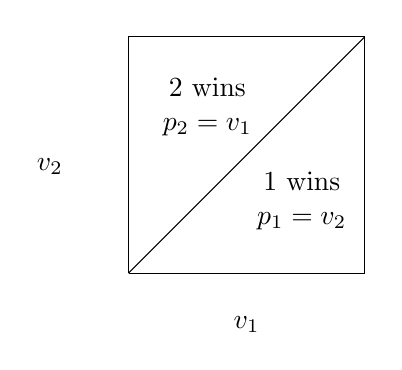
\begin{tikzpicture}
\draw (0,0) -- (3,0) node[label={[xshift=-1.5cm, yshift=-1cm]$v_1$}] {} -- (3,3) -- (0,3) -- (0,0)  node[label={[xshift=-1cm, yshift=1cm]$v_2$}] {};
\draw (0,0) -- (3,3)
node[label={[xshift=-2cm, yshift=-1cm]2 wins}] {}
node[label={[xshift=-2cm, yshift=-1.5cm]$p_2=v_1$}] {}
node[label={[xshift=-0.8cm, yshift=-2.2cm]1 wins}] {}
node[label={[xshift=-0.8cm, yshift=-2.7cm]$p_1=v_2$}] {}
;
\end{tikzpicture}
\end{center}

\begin{equation*}
    \begin{aligned}
        \mathbb{E}(\text{revenue})&=2\cdot\int_0^1\int_{v_2}^1 v_2 \d v_1 \d v_2\\
        &=2\cdot\int_0^1(1-v_2)v_2\d v_2\\
        &=2\left[\frac{1}{2}v_2^2-\frac{1}{3}v_2^3\right]_0^1=2\left[\frac{1}{2}-\frac{1}{3}\right]=\frac{1}{3}
    \end{aligned}
\end{equation*}

\end{document}


